% Chapter 3

\chapter{Data Integration} % Chapter title

\label{ch:dataintegration} % For referencing the chapter elsewhere, use \autoref{ch:mathtest}
%----------------------------------------------------------------------------------------
%
%----------------------------------------------------------------------------------------
To prepare for analytic work that is to be conducted in the thesis, an integrated knowledge base that has consistent and solid multivariate environmental data is developed from various data sources. It should be noted that these raw or derived products are of different data format and of different spatial resolution and temporal frequency.\\
\newline
To overcome this issue, Java\texttrademark~programming language's ease of cross-platform development and broad range of third-party libraries made it the choice of programming for data accessing, processing and integration in the work of this thesis.\\
\newline
In the rest of this chapter, each of the data sets is briefly introduced about its mission objectives, novelty and difference to other data sets, data availability in terms of spatial resolution and temporal frequency. In each of the sections, the Java implementation of accessing and preprocessing of the data are also explained via pseudo code where appropriate.
%-----------------------
\section{Australian Water Availability Project}
As mentioned in \autoref{subsection:dataavailability} \nameref{subsection:dataavailability}, the \ac{awap} is a joint effort contributed by \ac{cmar}, the \ac{bom} and the \ac{brs}\citep{Raupach2009}.\\
\newline
The AWAP aims to contribute to the overall understanding and monitoring of the Australian landscape systems, particularly the changes and feedback in climate, so that proper and robust management can be applied on a system-scale. It monitors the state and trend of the terrestrial water balance of the Australian continent.\\
\newline 
The approach it takes is based on model-data fusion, which is combining information from both the models and the data to maximise knowledge about the system. It contains historic and up-to-date data of soil moisture and all water influx and efflux contributing to changes in soil moisture (rainfall, transpiration, soil evaporation, surface runoff and deep drainage etc.), across Australia at a spatial resolution of 5 km. \\
\newline 
The AWAP data is available for access through a web interface, it provides three forms: (1) weekly near-real-time reporting, (2) historical monthly time series (1900 to present), and (3) monthly climatologies.\\
\begin{figure}[hbt]
\myfloatalign
\subfloat[{Precipitaion[mm/d]}]
{\label{fig:awapprec1}
\includegraphics[width=.45\linewidth]{gfx/awapprec}} \quad
\subfloat[{Percent Rank Precipitaion[\%]}]
{\label{fig:awapprec2}
\includegraphics[width=.45\linewidth]{gfx/awapprecper}}
\caption{Example of AWAP weekly near-real-time data. Date: 2014/02/17 to 2014/02/23. Acquired from CSIRO\citep{Awap2014}.}
\label{fig:awapprec}
\end{figure}
\newline
\autoref{fig:awapprec} shows an example of AWAP weekly data acquired from the web interface hosted by CSIRO. The example displays the precipitaion data in both physical values(\autoref{fig:awapprec1}) and percentage rank(\autoref{fig:awapprec2}) of the week from 2014/02/17 to 2014/02/23 on the Australian territories.
\subsection{Access and process AWAP data}
The weekly near-real-time reporting data is chosen among the three options above. As shown in \autoref{fig:awapflow1}, the data is accessed via the \ac{ftp} server provided by the \ac{eos} of CSIRO. This process is automated when the new data files become available on the remote FTP server. For any case study where the location of interest is given, the latitude and longitude can be entered as parameters to the module which returns the time series data of all AWAP variables. It is important to note that when parsing NetCDF format data files, the ones containing physical values of the environment variables should be used instead of percentage rank files, i.e. avoid using files that have characters \textbf{\emph{prc}} in the file names.\\
\begin{figure}[hbt] 
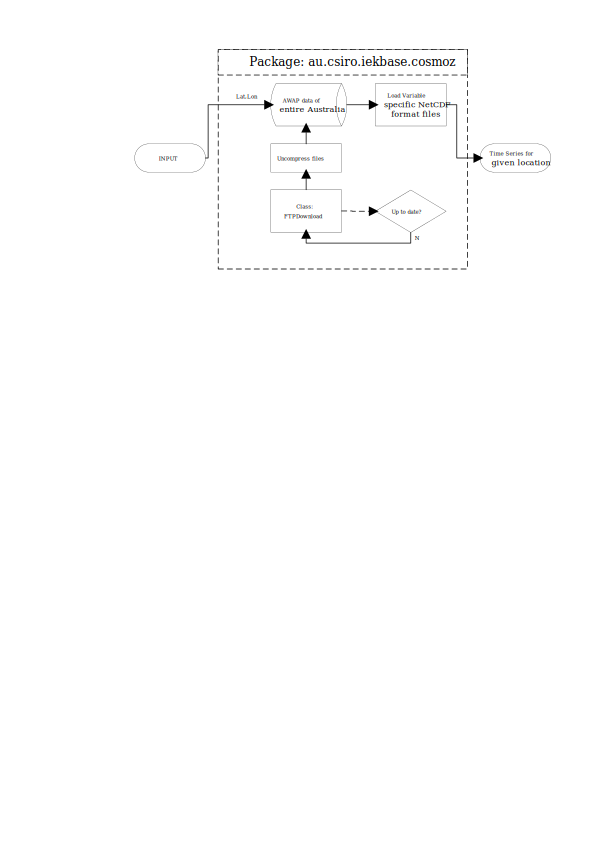
\includegraphics[width=1.1\linewidth]{gfx/awap1.jpg}
\caption{Implementation of AWAP Data Access and Process Module}
\label{fig:awapflow1}
\end{figure} 
\begin{figure}[hbt]
\includegraphics[width=1.1\linewidth]{gfx/awap2.jpg}
\caption{Batch Process of AWAP data for a rectangle region of interest}
\label{fig:awapflow2}
\end{figure} 
\newline
\autoref{fig:awapflow2} shows the case where a rectangle \ac{roi} is given and defined by the coordinate of its centre in latitude and longitude, the width and height of the rectangle. The required parameters can be calculated using the equations below.
\begin{align}
\text{latUL} &= \text{latC} + \frac{h}{2M}\\
\text{lonUL} &= \text{lonC} - \frac{w}{2M\cos(\pi\text{latC}/180)}
\end{align}
\begin{quote}
Where $\text{latUL}, \text{lonUL}$ are the latitude and longitude of the upper-left corner,\\
$\text{latC}, \text{lonC}$ are the latitude and longitude of the centre of the rectangle,\\
h and w are the height and width of the rectangle region of interest\\
and M is the constant equals to $111.111$.
\end{quote}
\autoref{fig:awapflow3} shows the detailed process of the method block \textbf{\emph{saveWeeklyData}} in \autoref{fig:awapflow2}. The method \textbf{\emph{createWeeklyData}} of class \emph{au.csiro.iekbase.integration.Initialization} utilises the native Java utility library \emph{java.util.Calendar} to find every Monday within the given time range, then creates folders following the naming convention ``YYY0MMDD-YYY1MMDD" where YYY0MMDD is the year, month and day of the current Monday and YYY1MMDD is the year, month and day of the following Sunday. The data are stored in \ac{csv} formatted files using the open source third party Java library \textbf{\emph{opencsv}}\citep{opencsv2014}.\\
\begin{figure}[hbt]
\includegraphics[width=1.1\linewidth]{gfx/awap3.jpg}
\caption{Detailed Process of Method: \emph{saveWeeklyData}}
\label{fig:awapflow3}
\end{figure} 

%-----------------------
\section{CosmOz: Australian National Cosmic Ray Soil Moisture Monitoring Facility} 
The \ac{cosmoz} is a near-real-time soil moisture measurement network provided by CSIRO, Monash University, Charles Darwin University and the University of New South Wales\citep{cosmoz2014}. It aims to test the utility of cosmic ray sensor system for water management, water information and hydrological process research applications, as well as to test the feasibility and utility of a national near-real time soil moisture measurement network. CosmOz also supports the evaluation of remote sensing products and hydrological models by expanding the set of soil moisture data available over Australia.\\
\newline
CosmOz currently has deployed 13 sensor systems at 12 locations across Australia, shown in \autoref{fig:cosmozloc}. Each CosmOz sensor system includes: 1* Hydroinnova CRS-1000 cosmic ray soil moisture sensor, 1* Hydrological Services tipping-bucket rain gauge, 3* Campbell TDR soil moisture probes and Quaesta data logger with integrated Iridium SBS satellite data communications.
\begin{figure}[hbt]
\myfloatalign
\subfloat[{Location of the 12 CosmOz monitoring sites. Acquired from University of Arizona\citep{arizona2014}}]
{\label{fig:cosmozloc}
\includegraphics[width=.52\linewidth]{gfx/cosmozloc}} \quad
\subfloat[{CosmOz system installed at Tullochgorum in Tasmania. Reprinted from ``{C}osm{O}z {W}iki Page'', by \citeauthor{cosmoz2014}, 2013. Copyright 2013 by \citeauthor{cosmoz2014}.}]
{\label{fig:cosmozphoto}
\includegraphics[width=.39\linewidth]{gfx/cosmozphoto}}
\caption{\ac{cosmoz} and one of its probes deployed in Tullochgorum site.}
\label{fig:cosmoz}
\end{figure}
\subsection{Access and pre-process CosmOz data}
The CosmOz data are provided by \citet{arizona2014} via its web server\footnote{COSMOS, University of Arizona\\ \url{http://cosmos.hwr.arizona.edu/}}. There is a data file of Microsoft Excel file(XLS) format available for each sensor location, updated every hour. An alternative data source is hosted by CSIRO\footnote{\url{http://southeskcosmoz.vm.csiro.au/}} as a backup server. The Java class \emph{CosmOz\_Data\_Preprocessor} of package \emph{au.csiro.iekbase.cosmoz} implements the access and pre-process methods of CosmOz data.
%-----------------------
\section{Landsat program}
The Landsat program is a joint effort of the \ac{usgs} and the \ac{nasa}. The Lantsat satellites have continuously acquired and delivered images of the Earth's land surface since 1972\citep{Mission2013}. The Landsat satellites have provided a valuable archive of space-based land remotely sensed data, contributed greatly in the studies of agriculture, geology, forestry, education, region planning, mapping and global change research. The simplified mission chronology is shown in \autoref{fig:landsat4decades}.\\
\begin{figure}[bth]
\begin{center}
\includegraphics[width=.95\linewidth]{gfx/landsat}
\end{center}
\caption{Overview of the Landsat program. Reprinted from ``Landsat: A Global Land-Imaging Mission'', by USGS, 2013. Copyright 2013 by USGS.  }
\label{fig:landsat4decades}
\end{figure}
\newline
Landsat 8 is the eighth and the latest Landsat satellite, launched on 11 February 2013. \autoref{table:landsatsum} details the eight Landsat satellites in terms of launch/decommission time, operation status and the sensors on-board respectively. In the ``Sensors'' column, Landsat 1,2,3 carries \ac{mss} and \ac{rbv}, Landsat 4,5 carries MSS and \ac{tm}, Landsat 6 carries \ac{etm}, Landsat 7 carries \ac{etm+} and Landsat 8 carries \ac{oli} and \ac{tirs}.\\
\begin{table}[hbt]
\caption{Details of Landsat missions. Adapted from ``Landsat: A Global Land-Imaging Mission'', by USGS, 2013. Copyright 2013 by USGS.}
\begin{center}
\rowcolors{2}{cyan!15}{white} 
\begin{tabular}{llll} 
\hline
\textbf{Satellite}&\textbf{Launch}&\textbf{Decommissioned}&\textbf{Sensors}\\
\hline
Landsat 1 & 23 July 1973 & 6 January 1978 & MSS/RBV \\
Landsat 2 & 22 January 1975 & 27 July 1983 & MSS/RBV \\
Landsat 3 & 5 March 1978 & 7 Septermber 1983 & MSS/RBV \\
Landsat 4 & 16 July 1982 & 15 July 2001 & MSS/TM \\
Landsat 5 & 1 March 1984 & 2013 & MSS/TM \\
Landsat 6 & 5 October 1993 & Did not achieve orbit & ETM\\
Landsat 7 & 15 April 1999 & Operational & ETM+ \\
Landsat 8 & 11 February 2013 & Operational & OLI/TIRS\\
\hline 
\end{tabular}
\end{center}
\label{table:landsatsum}
\end{table}
\newline
It is noteworthy that both Landsat 6 and Landsat 7 suffered from operational failures. Landsat 6 did not achieve its target orbit during the launching phase, thus it was officially declared as a failure by the \ac{noaa}\citep{Viets1995}. Landsat 7 experienced a failure in its \ac{slc} mechanism on 31 May 2003, which resulted in wedge-shaped scan-to-scan gaps. Which can be seen in \autoref{fig:l7slcoff}, comparing to \autoref{fig:l7slcon}, there are blank gaps on the image where data is not available.
\begin{figure}[hbt]
\myfloatalign 
\subfloat[{Landsat 7 Natural Color Image with SLC-ON. Captured on 9 January 2003.}]
{\label{fig:l7slcon}
\includegraphics[width=.45\linewidth]{gfx/l7slcon}} \quad
\subfloat[{Landsat 7 Natural Color Image with SLC-OFF (with gaps). Captured on 25 March 2007.}] 
{\label{fig:l7slcoff}
\includegraphics[width=.45\linewidth]{gfx/l7slcoff}}
\caption{Landsat 7 ETM+ images of the Tasmania south-eastern area captured before and after the SLC failure. Acquired from USGS.}
\label{fig:l7slc}
\end{figure}
\subsection{Access and pre-process Landsat data}
The Landsat data used in this study is accessed via the \emph{earthexplorer}\footnote{USGS EarthExplorer\\ \url{http://earthexplorer.usgs.gov/}} portal provided by USGS. The following procedures are performed to access and pre-process the raw data. In addition, refer to the \autoref{manual}, a graphic reference manual that explains how to setup a specific location-based multivariate database is completed for the work outlined in this thesis. 
\begin{enumerate}
  \item Location to Tile conversion.\\The georeference formats employed for the Landsat imagery include a \ac{utm} and a \ac{wgs84} datum and ellipsoid\citep{Johnson2013}. Therefore it is necessary to convert the location information to Landsat tiles which is in the form of a Path/Row combination.
  \item Select appropriate Landsat satellite imagery archive according to the desired time. As explained previously, not all Landsat satellites met their designed requirement, many of which had suffered from certain failure. To minimize the effort and inaccuracy introduced by artificially filling the gap of Landsat 7 SLC-OFF images, \autoref{table:landsatarchive} is referred to when selecting the appropriate imagery archive.
	\begin{table}[hbt]
	\caption{Table for selecting appropriate Landsat archive}
	\begin{center}
	\rowcolors{2}{cyan!15}{white} 
	\begin{tabular}{|l|lllll|} 
	\hline
	\textbf{Year}&1987-1999&2000-2003&2003-2009&2010-2013&2013-Now\\
	\hline
	\textbf{Archive}&L4\&5 & L7 SLC-ON & L5 & L7 SLC-OFF & L8 \\
	\hline 
	\end{tabular}
	\end{center}
	\label{table:landsatarchive}
	\end{table}
	
  \item The required Level 1 products are downloaded using the \ac{bda} program provided by USGS. The naming convention of level 1 products is \\
  \newline
  LXSPPPRRRYYYYDDDGSIVV
  \begin{quote}
  Where L = Landsat, X = Sensor, S = Satellite, PPP = WRS path, RRR = WRS row, YYYY = Year, DDD = Julian day of year, GSI = Ground station identifier and VV = Archive version number.
  \end{quote}
  \item Uncompress the data in a local directory, use the metadata (the filename contains \emph{\_MTL.txt}) provided in each of the level 1 product to acquire essential meterological information such as cloud cover, specific acquired time, date, azimuth angle and elevation etc.
  \item Batch process each of the band GeoTIFF files using the Java package, namely the class \emph{au.csiro.iekbase.landsat.Landsat\_parser} which uses the \textbf{GeoTools} open source Java library under GNU \ac{lgpl} license. The files contains \emph{\_BN.TIF} in its filenames, where \emph{N} is the band number as of each satellite's definition.\\ 
  The implementation of the Java class \emph{Landsat\_parser} is illustrated in \autoref{fig:landsatparser}.
	\begin{figure}[bth]
	\begin{center}
	\includegraphics[width=.95\linewidth]{gfx/landsat1}
	\end{center}
	\caption{Detailed Implementation of Class: \emph{Landsat\_parser}}
	\label{fig:landsatparser}
	\end{figure}
  \item Save the extracted Landsat Multi-Band data for the ROI in the same weekly manner as shown in \autoref{fig:awapflow3}.
\end{enumerate}
%-----------------------
\section{Moderate-resolution Imaging Spectroradiometer}
\ac{modis} is an instrument carried by Terra (EOS AM) and Aqua (EOS PM) satellites launched by NASA in 1999 and 2002 respectively\citep{Lindsey2013}. These two satellites orbit around the Earth every two days, and they are timed so that Terra passes from north to south across the equator in the morning while Aqua passes south to north over the equator in the afternoon. The aim of the MODIS program is to improve the understanding of global dynamics and processes occurring on the land, in the oceans and in the lower atmosphere, by acquiring remote sensing data in 36 spectral bands over the Earth surface. MODIS's frequent coverage complements other imaging systems such as
the Landsat, which reveals the Earth in finer spatial detail, however can only image a given area once every 16 days.
 \\
\newline 
MODIS provides a variety of derived products as well as raw data of different resolutions, based on the scientific algorithms which are detailed in their \acp{atbd}. The products have spatial resolution ranges from 250m to 5600m and temporal resolution ranges from daily to yearly.
\subsection{Access and pre-process MODIS data}
The MODIS data used in this study is accessed via the \emph{earthexplorer} portal provided by USGS. The following procedures are performed to access and pre-process the raw data. The reference manual as in \autoref{manual}, explains how to setup a specific location-based multivariate database is completed for the work outlined in this thesis. 
\begin{enumerate}
  \item Location to tile conversion. \\
The geo-reference system employed for the MODIS imagery is a sinusoidal tile grid, which is non-conventional thus requires specific reprojection process prior of use. The algorithm to perform such reprojection between latitude/longitude combination to sinusoidal grids is given by the MODIS Land Science Team\citep{modis2005}. Java Class \emph{au.csiro.iekbase.modis.MODIS\_reprojection} implemented the following formulas to perform such projection.
  \begin{quote}
  From latitude/longitude to sinusoidal tiles:
  \end{quote}
  \begin{align}
  y &= lat/rad2deg \\
  x &= lon/rad2deg \cdot \cos y\\
  \text{tileVertical} &= (\pi - y)/\text{tileSize}\\
  \text{tileHorizontal} &= (x+\pi)/\text{tileSize}\\
  \text{rowN} &=  ((\pi/2 - y)/\text{tileSize} - \text{tileVertical}) \cdot \text{nPixel} - 0.5\\
  \text{columnN} &= ((x+\pi)/\text{tileSize} - \text{tileHorizontal})\cdot \text{nPixel} - 0.5
  \end{align}
  \begin{quote}
  Where $rad2deg = 180/\pi$, $\text{tileSize} = 2\pi/36$ , $\text{nPixel} = 4800$ which is number of pixels in an axis, 4800 for 250m resolution.\\ And tileVertical/tileHorizontal is the tile combination for MODIS geo-reference system, rowN/columnN is the number of row and column on this specific tile that corresponds o the latitude/longitude combination that is provided.
  \end{quote}
  \item 
  Both Aqua and Terra \ac{vi} data are downloaded using the BDA program in a local directory for pre-processing. The naming convention of MODIS VI products is\\ \newline
  MYD13Q1.A2013233.h28v13.005.2013253050049
  \begin{quote}
  Where MYD13Q1 or MOD13Q1 are the product short names, A2013223 is the Julian date of acquisition (A-YYYYDDD), h28v13 is the Tile identifier, meaning 28th tile horizontally and 13th tile vertically, 005 is the collection version, 2013253050049 is the Julian date of production (YYYYDDDHHMMSS). 
  \end{quote}
  \item
  The MODIS data files are of the format HDF-EOS, which is developed specifically for the Earth Observation System of NASA. The Java package \emph{au.csiro.iekbase.modis} is developed utilising the Java HDF Object package provided by The HDF Group\citep{hdf2013}.\\ The implementation regards the HDF-EOS formatted files as general HDF4 formatted files and extract the \ac{ndvi} values for the ROI, which then being saved to the same weekly folders' structure, in the same manner as Landsat.
\end{enumerate}

%-----------------------
\section{National Elevation Data Framework}
The \ac{nedf} is developed to help Australia with the fundamental demands in tackling climate change, water management and various other dependent requirements\citep{Tickle2008}. NEDF provides \ac{ded} via a web portal which allows government and non-government clients to search and access to the specific data that is needed for their application.\\
\newline
The DED is generally available in most areas in three forms that suit different purposes: 
\begin{enumerate}
  \item \acp{dem} is a representation of continuous elevation values over a topographic surface by a regular array of sampled z-values, referenced to a common datum. The DEM is ground only representation and excludes vegetation such as trees and shrubs and human constructed features such as sheds and houses.
  \item \ac{dsm} includes ground, vegetation, building and structures.
  \item \ac{dtm} only represents the bare ground surface without any objects like plants and buildings.
\end{enumerate}
The DEDs that are accessable from NEDF web portal have various spatial resolutions, the commonly used resolutions are 9 seconds (approximately 250m), 3 seconds (approximately 100m) and 1 second (approximately 30m).
\subsection{Access and pre-process Elevation data}
The Digital Elevation data used in this study is accessed via the NEDF web portal\footnote{NEDF Portal\\\url{http://nedf.ga.gov.au/}}. The following procedures are performed to access and pre-process the data, of which the details are explained in the reference manual in \autoref{manual}.
\begin{enumerate}
  \item For the study in this thesis, the DEM is selected out of the three available forms of DED, as the major concern is to study the agricultural aspects of the land, which means that the buildings and structures are irrelevant information.
  \item The DEM data files are of the format ESRI\_GRID, which cannot be accessed directly using the intended software platform for analysis. Thus the data are converted to GeoTIFF format using \ac{envi} manually then the converted files can be parsed using a package \\\emph{au.csiro.iekbase.digitalElevationData} that is adapted from the class \emph{Landsat\_parser} which is mentioned previously.
  \item Note that the DED data is a one-off process unlike other data sets which has numerous data over the timespan of interest.
\end{enumerate} 
%-----------------------
\section{SILO}
SILO is an enhanced database of climate related information, solely provided by The Science Delivery Division of the \ac{dsitia}, which uses the historic data from BOM.\\
\newline
The SILO team's aim is to:
\begin{itemize}
  \item maintain and improve the quality of systems delivering historical data.
  \item incorporate climate change scenarios into the SILO dataset to allow the delivery of daily projections for 2030 and 2050 at any location in Australia.
  \item develop new ways to deliver climate change scenarios to help analyse climate change impacts and development of adaptation policy by SILO��s clients.
  \item raise awareness of SILO��s current and proposed services.
\end{itemize}
The SILO data contains 15 different climate variables, including temperature, rainfall, solar radiation etc. It is provided at a spatial resolution of 5km and on a daily frequency.
\subsection{Access and pre-process SILO data}
The SILO data are provided by the Long Paddock\footnote{The Long Paddock\\\url{https://www.longpaddock.qld.gov.au}} of the Queensland Government via an internally provided \ac{api}. For a given location, the integration program first determines the nearest available SILO sensor station, then request for the latest data file via the API. If successful, the data file would be returned in txt format. Java class \emph{SILO\_Data\_Preprocessor} of package \emph{au.csiro.iekbase.cosmoz} implements such methods.